\documentclass[11pt,a4paper]{ctexart}

\usepackage[margin=2.6cm]{geometry}
\usepackage{amsmath,amssymb,amsthm}
\usepackage{graphicx}
\usepackage{booktabs}
\usepackage{hyperref}
\usepackage{xcolor}
\usepackage{listings}
\usepackage{caption}

\graphicspath{{figures/}}
\hypersetup{colorlinks=true, linkcolor=blue!50!black, urlcolor=blue!60!black}
\lstset{
  basicstyle=\ttfamily\small,
  breaklines=true,
  frame=single,
  columns=fullflexible,
  backgroundcolor=\color{gray!7}
}

\newtheorem{definition}{定义}[section]
\newtheorem{theorem}{定理}[section]
\newtheorem{lemma}{引理}[section]
\newtheorem{proposition}{命题}[section]
\newtheorem{example}{例}[section]

\title{第 11 章 \quad Spectral Analysis / 谱分析}
\author{基于 \textit{A Course in Time Series Analysis} 的中文讲义与 Python 实践}
\date{}

\begin{document}
\maketitle

\section*{本章学习目标}

本章按照原文 \textit{Spectral Analysis} 的小节顺序整理，保留主要定义、定理、模型公式和练习方向，并将原文中的 R 实践思路改写为 Python 工程实践。

完成本章后，应能够：
\begin{itemize}
  \item 理解 DFT 和周期图的抽样分布；
  \item 掌握谱密度估计的滞后窗和平滑周期图方法；
  \item 理解 Whittle 似然及其与高斯似然的关系；
  \item 了解比率统计在时间序列中的作用；
  \item 进行线性模型拟合优度检验。
\end{itemize}

\section{DFT 与周期图}

周期图定义为
\[
  I_n(\omega)=\frac1n\left|\sum_{t=1}^n X_t e^{it\omega}\right|^2.
\]
\begin{lemma}[原文 Lemma 11.1.1]
在零均值二阶平稳和短记忆条件下，DFT 的二阶矩由谱密度近似控制，不同 Fourier 频率近似不相关。
\end{lemma}

周期图是谱密度的原始估计，但它本身不相合：样本量增大时方差并不自动消失。

\section{DFT 和周期图的分布}

对线性过程，在适当系数可和和矩条件下，
\[
  J_n(\omega_j)\approx \mathcal{CN}(0,2\pi f(\omega_j)),
\]
因此
\[
  \frac{I_n(\omega_j)}{2\pi f(\omega_j)}
\]
近似服从指数分布。原文用一系列引理和定理证明这一近似，并说明不同频率近似独立。

\section{谱密度估计}

\subsection{滞后窗估计}

用样本自协方差和窗口 \(w(\cdot)\) 可定义
\[
  \hat f(\omega)=\frac1{2\pi}\sum_{|k|\le m}w(k/m)\hat c(k)e^{-ik\omega}.
\]
窗口截断降低方差，但会引入偏差。

\subsection{平滑周期图}

另一种等价做法是在频域中平均邻近周期图：
\[
  \hat f(\omega)=\sum_j W_m(\omega-\omega_j)I_n(\omega_j).
\]
\begin{theorem}[谱估计抽样性质，原文 Theorem 11.3.1]
在平稳、短记忆和带宽条件下，平滑谱估计渐近无偏且方差随带宽增加而下降。
\end{theorem}

\section{Whittle 似然与比率统计}

Whittle 似然把 DFT 近似独立性用于参数估计：
\[
  L_W(\theta)=\sum_{\omega_j}
  \left\{\log f_\theta(\omega_j)+\frac{I_n(\omega_j)}{f_\theta(\omega_j)}\right\}.
\]
它近似高斯似然，但避免直接处理大型 Toeplitz 协方差矩阵。

\subsection{比率统计}

若把周期图与拟合谱密度作比
\[
  R(\omega_j)=\frac{I_n(\omega_j)}{f_{\hat\theta}(\omega_j)},
\]
模型拟合良好时，比率应近似白噪声频域形态。原文进一步讨论了基于比率的检验统计量。

\section{拟合优度检验}

线性时间序列模型拟合后，应检查残差和标准化周期图是否仍含系统性频率结构。谱域拟合优度检验与第 8 章的 ACF/Portmanteau 检验互为补充。

\section{原文小节覆盖补充}

\subsection{周期图分布的线性过程条件}
若 \(X_t=\sum_{j=0}^{\infty}\psi_j\varepsilon_{t-j}\) 且 \(\sum j^{1/2}|\psi_j|<\infty\)，则 DFT 渐近复正态，标准化周期图近似指数分布。

\begin{lemma}[线性过程 DFT，原文 Lemma 11.2.1--11.2.2]
线性过程的 DFT 可写为创新 DFT 乘以传递函数再加边界误差；在系数可和条件下边界误差可忽略。
\end{lemma}

\begin{proposition}[创新 DFT，原文 Proposition 11.2.1]
iid 创新的 DFT 在不同 Fourier 频率上渐近独立复正态，是一般线性过程结果的基础。
\end{proposition}

\begin{theorem}[周期图渐近分布，原文 Theorem 11.2.1]
在线性过程和矩条件下，不同 Fourier 频率处的周期图近似独立，且 \(I_n(\omega_j)/f(\omega_j)\) 近似指数型分布。
\end{theorem}

\subsection{滞后窗与谱窗例子}
Example 11.3.1 展示常见 lag windows。Example 11.3.2 展示 spectral windows。滞后窗估计在时域截断协方差，谱窗估计在频域平滑周期图。

\begin{lemma}[滞后窗期望，原文 Lemma 11.3.1]
谱估计的期望等于真实谱密度与谱窗的卷积，因此窗口宽度控制偏差和平滑程度。
\end{lemma}

\begin{lemma}[谱窗正则性，原文 Lemma 11.3.2]
若核函数有有界导数，则离散谱窗可稳定近似连续卷积，为渐近性质提供技术条件。
\end{lemma}

\subsection{Whittle 似然性质}
Example 11.4.1 给出 ARMA(1,1) 拟合。Whittle 似然衡量模型谱密度与周期图的匹配，避免直接处理大型 Toeplitz 协方差矩阵。

\begin{lemma}[Whittle 展开，原文 Lemma 11.4.1--11.4.3]
在因果 ARMA 和平滑条件下，Whittle 目标函数一致收敛，其导数展开可用于证明估计量一致和渐近正态。
\end{lemma}

\begin{theorem}[Whittle 渐近性质，原文 Theorem 11.4.1]
若模型正确且满足正则条件，Whittle 估计量渐近正态，极限方差由谱密度对参数的导数决定。
\end{theorem}

\subsection{比率统计和拟合优度}
第 11.5 节研究标准化周期图的比率统计。若模型拟合好，\(I_n(\omega)/f_{\hat\theta}(\omega)\) 不应呈现系统频率结构。Example 11.5.1 用 Whittle 似然说明该形式。第 11.6 节据此构造线性时间序列模型拟合优度检验，附录第 11.7 节给出技术引理。

\section{Python 工程实践}

在本章目录下运行：
\begin{lstlisting}[language=bash]
python scripts/ch11_generate_figures.py
\end{lstlisting}

脚本会把图像写入本章 \texttt{figures/} 目录。当前图像用于配合本章核心概念的仿真说明；若后续补齐原始数据文件，可把模拟数据替换为原文真实数据案例。

\begin{figure}[htbp]
  \centering
  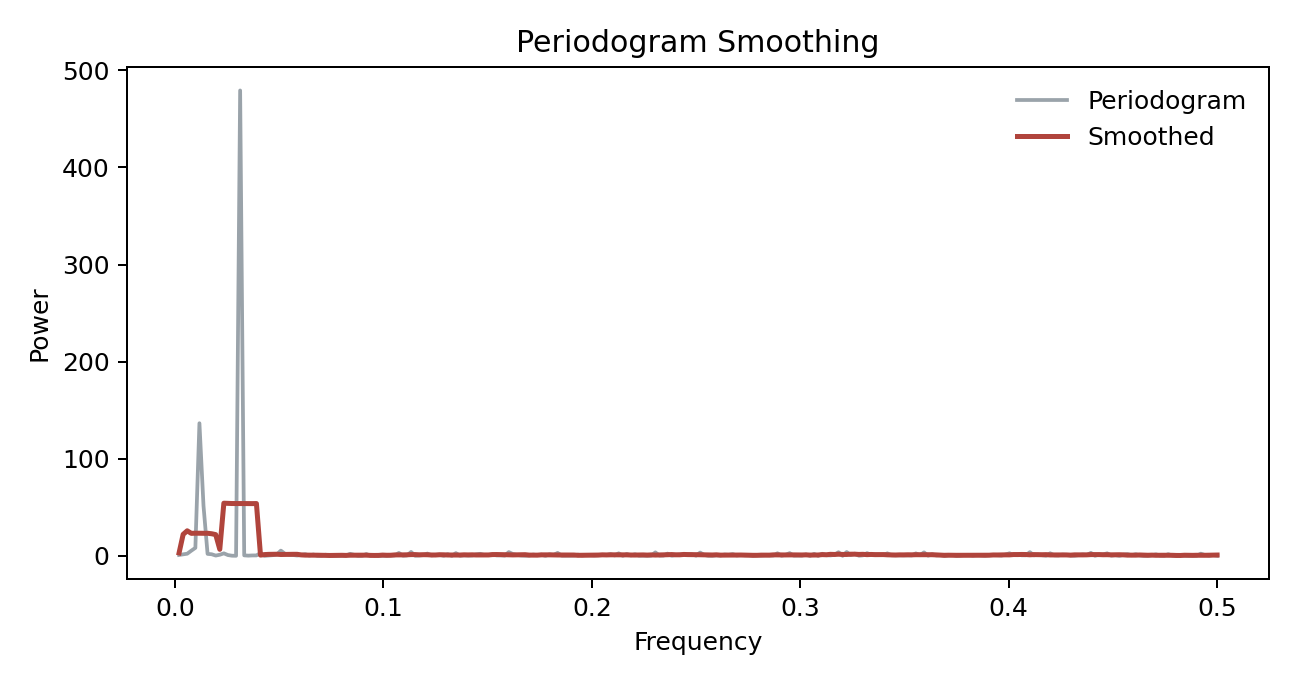
\includegraphics[width=0.86\textwidth]{ch11_fig01_smoothed_periodogram.png}
  \caption{周期图平滑：原始周期图方差大，平滑后更接近谱密度形状。}
\end{figure}

\begin{figure}[htbp]
  \centering
  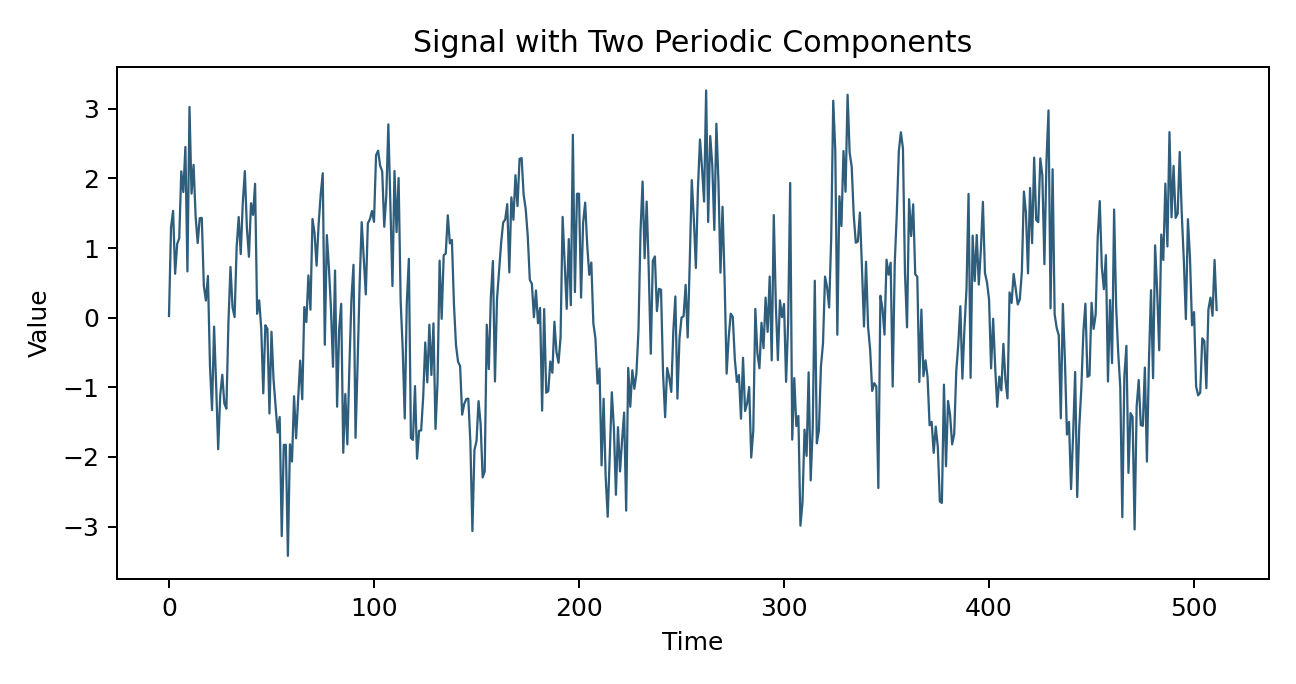
\includegraphics[width=0.86\textwidth]{ch11_fig02_two_frequency_signal.png}
  \caption{双频信号：时域叠加的周期成分会在频域形成多个峰。}
\end{figure}

\section{练习提要}

原文练习主要围绕下列方向展开：
\begin{itemize}
  \item 模拟线性过程并比较周期图与理论谱密度；
  \item 实现 Bartlett、Daniell 等平滑窗口；
  \item 用 Whittle 似然拟合 ARMA 模型；
  \item 基于标准化周期图检查模型拟合优度。
\end{itemize}

\section*{本章小结}

第 11 章从谱表示走向谱估计。周期图是入口但不相合，平滑和窗口提供稳定估计；Whittle 似然利用频域近似独立性，给出高效的参数估计和拟合检验工具。

\end{document}
